\providecommand{\main}{..}
\documentclass[\main/thesis.tex]{subfiles}
\begin{document}

\graphicspath{ {images/}{../images/} }

\chapter{Introduction}\label{introduction}

\section{Positional Numeral Systems}

A numeral system is a writing system for expressing numbers, and humans have
invented various kinds of numeral systems throughout history.
Take the number ``2016'' for example:

\begin{center}
    \begin{tabular}{ | l | r | }
    \textbf{Numeral system} & \textbf{notation}  \\
    \hline
    Chinese numerals    & 兩千零一十六    \\
    Roman numerals      & MMXVI         \\
    Egyptian numerals   & 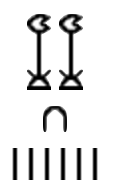
\includegraphics[width=2em]{egyptian/2016.png} \\
    \end{tabular}
\end{center}

Even so, most of the systems we are using today are positional notations\cite{knuth1998art}
because they can express infinite numbers with just a finite set of symbols called \textbf{digits}.

\subsection{Digits}

Any set of symbols can be used as digits as long as we know how to \textit{assign}
each digit to the value it represents.

\begin{center}
    \begin{adjustbox}{max width=\textwidth}
    \begin{tabular}{ | l | *{16}{l} | }
    \textbf{Numeral system} & \multicolumn{16}{c |}{\textbf{Digits} } \\
    \hline
    decimal         & 0 & 1 & 2 & 3 & 4 & 5 & 6 & 7 & 8 & 9 &    &    &    &    &    &    \\
    binary          & 0 & 1 &   &   &   &   &   &   &   &   &    &    &    &    &    &    \\
    hexadecimal     & 0 & 1 & 2 & 3 & 4 & 5 & 6 & 7 & 8 & 9 & A  & B  & C  & D  & E  & F  \\
    \hline
    \textbf{Assigned value}  & \textbf{0} & \textbf{1} & \textbf{2} & \textbf{3} & \textbf{4} & \textbf{5} & \textbf{6} & \textbf{7} & \textbf{8} & \textbf{9} & \textbf{10} & \textbf{11} & \textbf{12} & \textbf{13} & \textbf{14} & \textbf{15} \\
    \end{tabular}
    \end{adjustbox}
\end{center}

We place a bar above a digit to indicate its assignment.
For instance, these are the assignments of hexadecimal digits.

\begin{center}
    \begin{adjustbox}{max width=\textwidth}
    \begin{tabular}{ *{4}{c} }
    $ \bar{0} \mapsto 0 $ & $ \bar{1} \mapsto 1 $ & $ \bar{2} \mapsto 2 $ & $ \bar{3} \mapsto 3 $ \\
    $ \bar{4} \mapsto 4 $ & $ \bar{5} \mapsto 5 $ & $ \bar{6} \mapsto 6 $ & $ \bar{7} \mapsto 7 $ \\
    $ \bar{8} \mapsto 8 $ & $ \bar{9} \mapsto 9 $ & $ \bar{A} \mapsto 10 $ & $ \bar{B} \mapsto 11 $ \\
    $ \bar{C} \mapsto 12 $ & $ \bar{D} \mapsto 13 $ & $ \bar{E} \mapsto 14 $ & $ \bar{F} \mapsto 15 $ \\
    \end{tabular}
    \end{adjustbox}
\end{center}

Positional numeral systems represent a number by lining up a series of digits:

$$ \xrightarrow{2016} $$

In this case, $ 6 $ is called the \textit{least significant digit},
and $ 2 $ is known as the \textit{most significant digit}.
Except when writing decimal numbers,
we will write down numbers in reverse order,
from the least significant digit to the most significant digit like this

$$ \xleftarrow{6102} $$

\subsection{Syntax and Semantics}

Syntax bears no meaning;
its semantics can only be expressed through the process of \textit{converting} to some other syntax.
Numeral systems are merely syntax.
The same notation can represent different numbers in different context.

Take the notation "11" for example; it could have several meanings.

\begin{center}
    \begin{tabular}{ | l | r | }
    \textbf{Numeral system}      & \textbf{number in decimal}  \\
    \hline
    decimal             & 11    \\
    binary              & 3     \\
    hexadecimal         & 17    \\
    \end{tabular}
\end{center}

To make things clear, we call a sequence of digits a \textbf{numeral}, or \textbf{notation};
the number it expresses a \textbf{value}, or simply a \textbf{number};
the process that converts notations to values an \textbf{evaluation}.
From now on, \textbf{numeral systems} only refer to the positional ones.
We will not concern ourselves with other kinds of numeral systems.

\subsection{Evaluating Numerals}

What we mean by a \textit{context} in the previous section is the \textbf{base}
of a numeral system.
The ubiquitous decimal numeral system as we know has the base of 10,
while the binaries that can be found in our machines nowadays has the base of 2.

\begin{center}
    \begin{adjustbox}{max width=\textwidth}
    \begin{tabular}{ | l | l | *{16}{l} | }
    \textbf{Numeral system} & \textbf{Base}  & \multicolumn{16}{c |}{\textbf{Digits} } \\
    \hline
    decimal         & 10 & 0 & 1 & 2 & 3 & 4 & 5 & 6 & 7 & 8 & 9 &    &    &    &    &    &    \\
    binary          & 2  & 0 & 1 &   &   &   &   &   &   &   &   &    &    &    &    &    &    \\
    hexadecimal     & 16 & 0 & 1 & 2 & 3 & 4 & 5 & 6 & 7 & 8 & 9 & A  & B  & C  & D  & E  & F  \\
    \hline
    \textbf{Assigned value}  & & \textbf{0} & \textbf{1} & \textbf{2} & \textbf{3} & \textbf{4} & \textbf{5} & \textbf{6} & \textbf{7} & \textbf{8} & \textbf{9} & \textbf{10} & \textbf{11} & \textbf{12} & \textbf{13} & \textbf{14} & \textbf{15} \\
    \end{tabular}
    \end{adjustbox}
\end{center}


A numeral system of base $n$ has exactly $n$ digits, which are assigned values
from $0$ to $n-1$.

Conventionally, the base of a system is annotated by subscripting it to the
right of a numeral, like $ ({2016})_{10} $.
We replace the parenthesis with a fancy pair of semantics brackets,
like $ [\![ 2016 ]\!]_{10} $ to emphasize its role as the evaluation function.

To evaluate a notation of a certain base:
$$
    [\![d_0d_1d_2...d_n]\!]_{base}
    =
    \bar{d_0}\times base^0 + \bar{d_1}\times base^1 + \bar{d_2}\times base^2 + ... + \bar{d_n}\times base^n
$$

Where $ d_{n} $ is a digit for all $ n $.

\section{Unary Numbers and Peano Numbers}

Some computer scientists and mathematicians seem to be more comfortable with
unary (base-1) numbers because they are isomorphic to the natural numbers à la Peano.

$$
    [\![1111]\!]_{1} \cong
        \overbrace{\text{suc (suc (suc (suc}}^4 + \text{ zero)))}
$$

Statements established on such construction can be proven using mathematical
induction. Moreover, people have implemented and proven a great deal of functions
and properties on these unary numbers because they are easy to work with.

However, if we are to evaluate unary numerals with the model we have just settled,
the only digit of the unary system would have to be assigned to $ 0 $ and
every numeral would evaluate to zero as a result.

\paragraph{problem}
The definition of digit assignments can be modified to allow unary digits to
start counting from $ 1 $, but that would lead to inconsistency among systems
of other bases.

\begin{center}
    \begin{adjustbox}{max width=\textwidth}
    \begin{tabular}{ | l | l | *{16}{l} | }
    \textbf{Numeral system} & \textbf{Base}  & \multicolumn{16}{c |}{\textbf{Digits} } \\
    \hline
    decimal         & 10 & 0 & 1 & 2 & 3 & 4 & 5 & 6 & 7 & 8 & 9 &    &    &    &    &    &    \\
    binary          & 2  & 0 & 1 &   &   &   &   &   &   &   &   &    &    &    &    &    &    \\
    hexadecimal     & 16 & 0 & 1 & 2 & 3 & 4 & 5 & 6 & 7 & 8 & 9 & A  & B  & C  & D  & E  & F  \\
    unary           & 1  &   & 1 &   &   &   &   &   &   &   &   &    &    &    &    &    &    \\
    \hline
    \textbf{Assigned value}  & & \textbf{0} & \textbf{1} & \textbf{2} & \textbf{3} & \textbf{4} & \textbf{5} & \textbf{6} & \textbf{7} & \textbf{8} & \textbf{9} & \textbf{10} & \textbf{11} & \textbf{12} & \textbf{13} & \textbf{14} & \textbf{15} \\
    \end{tabular}
    \end{adjustbox}
\end{center}

Moreover, theorems developed on natural numbers à la Peano cannot be migrated
to numbers of other representations, although the proofs are mostly identical.

\section{Binary Numerals in Digital Circults}

Recall how arithmetics such as long addition are performed by hand.

\begin{center}
    \begin{tabular}{c@{\,}c@{\,}c@{\,}c}
      & 1 & 2 & 3 \\
    + &   & 3 & 4 \\
    \hline
      & 1 & 5 & 7 \\
    \end{tabular}
\end{center}

The greater a number is, the longer its notation will be, which in terms
determines the time it takes to perform operations.
Since a system can only have \textbf{finitely many} digits, operations such as
addition on these digits must be \textbf{constant time}.
Consequently, the time complexity of operations such as long addition on a
numeral would be $ O(lg n) $ at best.
The choice of the base is immaterial as long as it is not unary
(which would degenerate to $ O(n) $).

However, this is not the case for the binary numeral system implemented in
arithmetic logic units (ALU). These digital circuits are designed to perform
fast arithmetics. Regarding addition, it takes only \textit{constant time}.

It seems that either we have been doing long addition wrong since primary school,
or the chip manufacturers have been cheating all the time. But there's a catch!
Because we are capable of what is called \textit{arbitrary-precision arithmetic},
i.e., we could perform calculations on numbers of arbitrary size
while the binary numbers that reside in machines are bounded by the hardware,
which could only perform \textit{fixed-precision arithmetic}.

\paragraph{problem}
Judging from the time complexity of operations, the binary numerals running in
digital circuits is certainly different from the ordinary binary numerals we have
known.

\section{Numerical representation}

\paragraph{lists and unary numbers}

One may notice that the structure of unary numbers looks suspiciously similar
to that of lists'. Let's compare their definition in Haskell.

\noindent\begin{minipage}{.45\textwidth}
\begin{lstlisting}
data Nat = Zero
         | Suc Nat
\end{lstlisting}
\end{minipage}\hfill
\begin{minipage}{.48\textwidth}
\begin{lstlisting}
data List a = Nil
            | Cons a (List a)
\end{lstlisting}
\end{minipage}

If we replace every {\lstinline|Cons _|} with {\lstinline|Suc|} and
{\lstinline|Nil|} with {\lstinline|Zero|}, then a list becomes an unary number.
This is precisely what the {\lstinline|length|} function,
a homomorphism from lists to unary numbers, does.

\tikzset{
    one/.style = {draw, circle, inner sep=0pt, minimum size=10pt, fill=black},
    zero/.style = {draw, circle, inner sep=0pt, minimum size=10pt},
    cons/.style = {draw, circle, inner sep=0pt, minimum size=25pt, font=\scriptsize},
    nil/.style = {draw, rectangle, inner sep=0pt, minimum size=20pt, font=\scriptsize},
    txt/.style = {circle}
}

\begin{center}
    \begin{tikzpicture}[edge from parent/.style = {draw, -latex}]
        \node[cons]{cons}
            child[grow=right] {node[cons]{cons}
                child[grow=right] {node[cons]{cons}
                    child[grow=right] {node[cons]{cons}
                        child[grow=right] {node[nil]{nil}
                            child[grow=down] {node[txt]{zero} edge from parent[-, dashed]}
                        }
                        child[grow=down] {node[txt]{suc} edge from parent[-, dashed]}
                    }
                    child[grow=down] {node[txt]{suc} edge from parent[-, dashed]}
                }
                child[grow=down] {node[txt]{suc} edge from parent[-, dashed]}
            }
            child[grow=down] {node[txt]{suc} edge from parent[-, dashed]};
    \end{tikzpicture}
\end{center}

Now let's compare addition on unary numbers and merge (append) on lists:

\noindent\begin{minipage}{.45\textwidth}
\begin{lstlisting}[basicstyle=\ttfamily\scriptsize]
add : Nat → Nat → Nat
add Zero    y = y
add (Suc x) y =
    Suc (add x y)
\end{lstlisting}
\end{minipage}\hfill
\begin{minipage}{.48\textwidth}
\begin{lstlisting}[basicstyle=\ttfamily\scriptsize]
append : List a → List a → List a
append Nil         ys = ys
append (Cons x xs) ys =
    Cons x (append xs ys)
\end{lstlisting}
\end{minipage}

Aside from having virtually identical implementations, operations on unary numbers
and lists both have the same time complexity. Incrementing a unary number takes
$ O(1) $, inserting an element into a list also takes $ O(1) $; adding two unary
numbers takes $ O(n) $, appending a list to another also takes $ O(n) $.

\paragraph{binomial heaps and binary numbers}

If we look at implementations and operations of binary numbers and binomial
heaps, the resemblances are also uncanny.

\begin{center}
    \begin{tikzpicture}[
        edge from parent/.style = {draw, -latex},
        node distance=40pt
    ]
        \node[one] (A) {}
            child[grow=up] {node[txt]{1} edge from parent[-, dashed]}
            child[grow=right] {node[zero] (B) {}
                child[grow=up] {node[txt]{0} edge from parent[-, dashed]}
                child[grow=right] {node[one, xshift=40pt] (C) {}
                    child[grow=up] {node[txt]{1} edge from parent[-, dashed]}
                    child[grow=down] {node[one] (C-1) {}}
                    child {node[one, left of = C-1] {}
                        child[grow=down] {node[one]{}}
                    }
                    child[grow=right] {node[one, xshift=120pt] (D) {}
                        child[grow=up] {node[txt]{1} edge from parent[-, dashed]}
                        child[grow=down] {node[one] (D-1) {}}
                        child {node[one, left of = D-1] (D-2) {}
                            child[grow=down] {node[one]{}}
                        }
                        child {node[one, left of = D-2] (D-3) {}
                            child[grow=down] {node[one] (D-3-1) {}}
                            child {node[one, left of = D-3-1] {}
                                child[grow=down] {node[one]{}}
                            }
                        }
                    }
                }
            };
    \end{tikzpicture}
\end{center}

The figure above is a binomial heap containing $ 13 $ elements.
\footnote{Nodes that contain elements are painted black.}
From left to right, there are \textit{binomial trees} of different \textit{ranks}
attached to the path that we call \textit{``the spine''}.
A binomial heap is composed of binomial trees just as a numeral is composed
of digits. If we read the nodes with binomial trees as $ 1 $ and those without
as $ 0 $, then we get the numeral of $ 13 $ in binary.

\paragraph{building blocks}

Single cells in lists and binomial trees in binomial heaps are all different
kind of simple data structures that are called \textit{building blocks}.
There are also other kinds of building blocks, such as perfect leaf trees.

\begin{center}
    \begin{tikzpicture}[
        edge from parent/.style = {draw, -latex},
        level/.style={sibling distance = 80pt/#1},
        level distance = 20pt
    ]
        \node[zero]{}
            child {node[zero]{}
                child {node[zero]{}
                    child {node[one]{}}
                    child {node[one]{}}
                }
                child {node[zero]{}
                    child {node[one]{}}
                    child {node[one]{}}
                }
            }
            child {node[zero]{}
                child {node[zero]{}
                    child {node[one]{}}
                    child {node[one]{}}
                }
                child {node[zero]{}
                    child {node[one]{}}
                    child {node[one]{}}
                }
            };
    \end{tikzpicture}
\end{center}

These building blocks can have different ranks.
A binary leaf tree of rank n, for instance, would contain $ 2^n $ elements.
The data structures we have addressed so far are all composed of a series of
building blocks that are ordered by their ranks.

However, these building blocks do not necessarily have to be binary based,
as long as multiple building blocks of the same rank can be merged into a
building block of a higher rank or vice versa.


\paragraph{random access lists and binary numbers}

Accessing an element on lists typically takes $ O(n) $.
Instead of using single cells, \textit{random access lists} adopts perfect
leaf trees as building blocks.
This improves the time complexity of random access from $ O(n) $ to $ O(lg n) $
as a random access list would have at most $ O(lg n) $ building blocks, and
the tallest perfect leaf tree takes at most $ O(lglg n) $ to traverse.

\tikzset{
    cltree/.style = {draw,
        font=\scriptsize,
        isosceles triangle, shape border rotate=90}
}
\begin{center}
    \begin{tikzpicture}[
        edge from parent/.style = {draw, -latex},
        node distance = 60pt
    ]
        \node[one](A){}
            child {node[zero, right of = A](B){}
                child {node[one, right of = B](C){}
                    child {node[one, right of = C](D){}
                        child {
                            node[cltree, scale=2.8, yshift=-5pt] {8} edge from parent[draw=none]
                        }
                        { node[cltree, scale=2] {4} }
                    }
                }
                { node[cltree, scale=1, yshift=20pt] {1} }
            };
    \end{tikzpicture}
\end{center}

Similar to that of binomial heaps, random access lists also have spines.
Also, treating building blocks as digits also yields binary numerals of the
container's size.

\subsection{The correspondence}

The strong analogy between data structures and positional numeral systems
suggests that numeral systems can serve as templates for designing containers.
Such data structures are called \textbf{Numerical Representations}\cite{okasaki1996purely}
\cite{hinze1998numerical}.

\begin{center}
    \begin{adjustbox}{max width=\textwidth}
    \begin{tabular}{ l l l }
    a container of size $ n $ & corresponds to & a numeral of $ n $ \\
    a building block of rank $ n $ & corresponds to & a digit of weight $ base^n $ \\
    inserting an element      & corresponds to & incrementing a numeral \\
    merging two containers    & corresponds to & adding two numerals \\
    \end{tabular}
    \end{adjustbox}
\end{center}

\paragraph{problem}

Retrieving the first element ({\lstinline|head|}) of a list typically takes
only constant time. On the other hand, it takes $ O(lg n) $ on random access lists.
To illustrate the problem, consider a random access list with $ 32 $ elements:

\begin{center}
    \begin{tikzpicture}[
        edge from parent/.style = {draw, -latex},
        node distance = 60pt
    ]
        \node[zero]{}
            child[grow=up] {node[txt]{0} edge from parent[-, dashed]}
            child[grow=right] {node[zero]{}
                child[grow=up] {node[txt]{0} edge from parent[-, dashed]}
                child[grow=right] {node[zero]{}
                    child[grow=up] {node[txt]{0} edge from parent[-, dashed]}
                    child[grow=right] {node[zero]{}
                        child[grow=up] {node[txt]{0} edge from parent[-, dashed]}
                        child[grow=right] {node[zero]{}
                            child[grow=up] {node[txt]{0} edge from parent[-, dashed]}
                            child[grow=right] {node[one]{}
                                child[grow=up] {node[txt]{1} edge from parent[-, dashed]}
                                { node[cltree, scale=1, yshift=-20pt] {32} }
                            }
                        }
                    }
                }
            };
    \end{tikzpicture}
\end{center}

To access any elements from the list above, we have to skip
through four empty nodes before reaching the first building block.
Nodes that correspond to the digit ``0'' contain no elements.
They are not only ineffective but also hinders traversal.

However, if we replace the digits ``0'' and ``1'' with ``1'' and ``2'',
then the number $ 32 $ can be represented as $ 21111 $ instead of $ 000001 $.
By doing so, we eliminate empty nodes and shorten the spine, thus improving
the performance of list traversal.

\begin{center}
    \begin{tikzpicture}[
        edge from parent/.style = {draw, -latex},
    ]
        \node[one](root){}
            child[grow=up] {node[txt]{2} edge from parent[-, dashed]}
            child[grow=right] {node[one]{}
                child[grow=up] {node[txt]{1} edge from parent[-, dashed]}
                child[grow=right] {node[one]{}
                    child[grow=up] {node[txt]{1} edge from parent[-, dashed]}
                    child[grow=right] {node[one]{}
                        child[grow=up] {node[txt]{1} edge from parent[-, dashed]}
                        child[grow=right] {node[one]{}
                            child[grow=up] {node[txt]{1} edge from parent[-, dashed]}
                            { node[cltree, scale=2, yshift=-25pt] {16} }
                        }
                        { node[cltree, scale=1.68, yshift=-23pt] {8} }
                    }
                    { node[cltree, scale=1.41, yshift=-22pt] {4} }
                }
                { node[cltree, scale=1.19, yshift=-21pt] {2} }
            }
            child {node[txt, below right = 16pt and 11pt of root]{}
                { node[cltree, scale=0.8, below right = 28pt and 5pt of root] {1} }
            }
            child {node[txt, below left = 16pt and 11pt of root]{}
                { node[cltree, scale=0.8, below left = 28pt and 5pt of root] {1} }
            };
    \end{tikzpicture}
\end{center}

The data structure introduced above is called the \textit{1-2 random access list}.
Its presence suggests that a binary numeral system with digits ``1'' and ``2''
should be admissible.

Hinze argues\cite{hinze1998numerical} that if we add the digit ``0'' back to the
\textit{1-2 random access list}, then the resulting numerical representation,
so-called \textit{0-1-2 random access list},
would even have a better performance of insertion and deletion in certain edge cases.

To accommodate these numerical representations, we need a more versatile
representation for numeral systems.

\section{Motivation and Outline}

We started off with numerical representations, but then we found that their
corresponding numeral systems alone are interesting enough.

\begin{itemize}
    \item How to capture the numeral systems behind these data structures?
    \item What are these numeral systems capable of?
    \item Which kind of numeral systems are suitable for modelling numerical
        representations? Do they support increment (insertion) or addition (merge)?
    \item What are the relations between these numeral systems and the natural numbers?
\end{itemize}

The remainder of the thesis is organized as follows.

\begin{description}
    \item[Chapter~\ref{generalizations}]
        resolves the problems we have addressed in this chapter by proposing
        some generalizations to the conventional positional numeral systems.
   \item[Chapter~\ref{agda}]
        gives a introduction to \textit{Agda}, the language we use to construct
        and reason about the representation.
   \item[Chapter~\ref{props}]
        introduces \textit{equational reasoning} and relevent properties
        of natural numbers used in the coming chapters.
   \item[Chapter~\ref{constructions}] constructs the representation for these
        numeral systems, defines operations such as increment and addition,
        search for suitable systems for modelling data structures,
        and examime the relations between these systems and the natural numbers.
    \item[Chapter~\ref{}] migrates propositions and proofs from the natural
        numbers à la Peano to our presentation of numbers.
    \item[Chapter~\ref{}] concludes everything.
\end{description}


% =======
% However, conventional numeral systems is incapable of modelling these numerical
% representations \scm{why not? Some brief explanation?}. Instead, we need a more versatile numeral system.
%
% \scm{You raised several potential questions in this chapter, for example:
% inconsistency between unary and other representations, inconsistency
% between ALU and arbitrary precision arithmetics, needing a more versatile
% numeral system, etc. However, it is not clear where all these questions
% lead to, and what you are trying to achieve in this thesis.
%
% It might help adding a section summarising what you did (and how that
% relates to the questions above). It also helps to give an outline of this thesis,
% so the readers would know what to expect in each chapters of this thesis.
% }
% >>>>>>> b542c5f8d1eefb58159d3ae7438f53ce219d9997
% [say something about redundant data structures]

% 1. RAL {0, 1}, {1, 2}, {1, 2, 3}

% Surprisingly, we could fit these binary numbers into our representation with
% just a tweak. If we allow a system to have more digits, then a fixed-precision
% binary number can be regarded as a single digit! To illustrate this, a 32-bit
% binary number would become a single digit that ranges from $ 0 $ to $ 2^{32} $,
% while everything else including the base remains the same.
%
% Formerly in our representation, there are exactly \textit{base} number of digits
% that range from:
%
% $$
%     \text{offset}  ...  \text{offset} + \text{base} - 1
% $$
%
% We introduce a new index \textit{\#digit} to generalize the number of digits.
% Now they range from:
%
% $$
%     \text{offset}  ...  \text{offset} + \text{\#digit} - 1
% $$
%
% Here's a table of the configurations about the systems that we've addressed:
%
% \begin{center}
%     \begin{tabular}{l*{3}{r}}
%     Numeral system      & base  & \#digit    & offset    \\
%     \hline
%     Decimal             & 10    & 10        & 0         \\
%     Binary              & 2     & 2         & 0         \\
%     Unary               & 1     & 1         & 1         \\
%     Int32               & 2     & $ 2^{32} $ & 0        \\
%     \end{tabular}
% \end{center}
%
% Consider this numeral system, the oridinary binary numbers with an extra digit:
% $ 2 $.
%
% \begin{center}
%     \begin{tabular}{l*{3}{r}}
%     Numeral system      & base  & \#digit    & offset    \\
%     \hline
%     0-1-2 Binary        & 2     & 3          & 0         \\
%     \end{tabular}
% \end{center}
%
% \begin{center}
%     \begin{tabular}{c*{1}{l}}
%     Number (in decimal)  & Notation \\
%     \hline
%     0       & 0 \\
%     1       & 1 \\
%     2       & 01, 2 \\
%     3       & 11 \\
%     4       & 001, 21 \\
%     5       & 101, 12 \\
%     \end{tabular}
% \end{center}
%
% Such a numeral system is said to be \textbf{redundant}, because there are more than one
% way to represent a number. In fact, systems that allow $ 0 $ as one of the digits
% must be redundant, since we can always take a number and add leading zeros without
% changing it's value. Systems that does not have zeros are said to be \textbf{zeroless}.
%
% We will see that there's a deep connection between data
% structures and  numeral systems. Data structures modeled after redundant numeral
% systems have some interesting properties.
%
%
% % \subsubsection{From numeral systems to numbers}
%
% % But that simplicity comes at a cost, the time complexity of functions defined on
% % unary numbers is significantly
%
% % People have implemented and proven a great deal of functions and properties on
% % these unary numbers because they are easy to work with. But the simplicity comes
% % at a cost, the time complexity of functions defined on unary numbers is significantly
% % higher than those defined on systems of other bases, say, binary numbers. Hence,
% % it's not practical in doing heavy calculations.
%
% % The \textit{numbers} we are constructing in this work are the \textit{natural numbers}.
% % We learned how to count with these numbers when we are little. But what are numbers, really?
%
% % \paragraph{Recursive}
%
% % Paul Benacerraf once argued\cite{benacerraf1965numbers} that, there are two kinds
% % of \textit{counting} which corresponds to \textbf{transitive} and \textbf{intransitive}
% % uses of the verb "to count". Transitive counting, in his sense, is to assign one
% % of the numbers to the cardinality of a set, by establish a one-to-one correspondence
% % between the numbers and the objects one is counting, all the way from none to
% % all. Intransitive counting, on the other hand, is to generate a sequence of
% % notation, that could go as far as we need. And it seems that one can only learn
% % how to count intransitively first, before knowning how to count transitively,
% % but not vice versa.
% %
% % He further discussed that the numbers must be at least recursive
%
% % \paragraph{Numbers are recursive}
% %
% % \paragraph{Internal definition is immaterial}
%
\end{document}
